\section{Neuronale Netzwerke}

\subsection{Geschichte}

Im Jahr 1943 wurde die erste Arbeit darüber geschrieben, wie Neuronen im Gehirn funktionieren könnten und die Autoren Warren McCulloch und Walter Pitts experimentierten sogar damit diese mit elektronischen Schaltkreisen nachzubauen.\footnote{\cite[]{alogicalcalculus}}

In den 1950er Jahren haben Forscher von IBM daran gearbeitet ein Neuronales Netzwerk mit einem Computer zu simulieren. Der Versuch scheiterte allerdings.\footnote{\cite[Absatz 3]{nnhistory}}

Immer wieder gab es kleinere Forschungsprojekte, ein sehr großer Durchbruch war aber 1975 die Entwicklung eines "`Backpropagation"' Algorithmus durch den Wissenschaftler Paul Werbos. Ähnliche Algorithmen wurden wiederholt und unabhängig entwickelt, aber Werbos' Algorithmus war der erste mit großer Bedeutung.\footnote{\cite[]{paulwerbosbackpropagation}} Das Prinzip des Algorithmus wird auch heute noch verwendet, es ist dieser Algorithmus der dem Neuronalen Netzwerk das selbstständige Lernen ermöglicht.\footnote{Genaueres in Kapitel \ref{funktionsweise}}

In 1998 veröffentlichte Yann LeCun und sein Team eine Arbeit über die Anwendung eines "`Convolutional Neural Networks\footnote{Ab jetzt als CNN bezeichnet}"' zur Erkennung von geschriebenen Zeichen in einem Dokument.\footnote{\cite[]{cnnhistory}} Diese Arbeit gilt als Ursprung des, für beispielsweise Bilderkennungs Software gut geeignete, CNNs und Weiterentwicklungen werden auch heute noch verwendet.

Obwohl ein großes Potenzial erkannt wurde, war es über die nächsten Jahre wieder recht still. Der nächste große Durchbruch passierte in 2012 als Geoffrey Hinton ein Modell entwickelte, was die Fehlerquote in einer öffentlichen Challenge für Bilderkennung beinahe halbierte.\footnote{\cite[]{geoffrey}} Der Grund dafür waren mehrere fundamentale Neuerungen aus dem Bereich Deep Learning; die wahrscheinlich größte Änderung: Starke Parallelisierung des Backpropagation-Prozesses, durch Verschiebung der Last von der CPU auf die GPU. Aufgrund der starken Überlegenheit eines Grafikprozessors in parallelisierten Prozessen, wie die benötigten Tensormultiplikationen durch die deutlich größere Anzahl an (dafür schwächeren) Kernen im Vergleich zu einer herkömmlichen CPU, kann ein Neuronales Netzwerk mehrere hundertmal schneller trainiert werden.

Heute gibt es (vergleichsweise) simple Frameworks, wie das im Jahr 2015 erschienende TensorFlow oder PyTorch aus 2016, welche das erstellen, trainieren und verwenden von Neuronales Netzwerk enorm vereinfachen. Ihr Funktionsumfang wächst durch die große Open-Source Community ständig.

%Sind die Zitate okay?

\begin{figure}[h]
    \begin{chronology}[10]{1940}{2020}{\textwidth}
        \event{1943}{Erste Arbeit und Experimente}
        \event[1950]{1960}{Bemühungen, ein NN\footnote{Kurzform für "`Neuronales Netzwerk"'} digital umzusetzen}
        \event{1975}{Backpropagation Algorithmus}
        \event{1998}{Erfindung des CNNs}
        \event[2015]{2020}{Entwicklung versch. Frameworks}
    \end{chronology}
    \caption[Zeitstrahl]{Zeitstrahl von 1940 bis 2020 mit den wichtigsten Ereignissen der Entwicklung künstlicher Neuronaler Netzwerke}
\end{figure}

\subsection{Aufbau}

\begin{wrapfigure}{r}{87mm}
    
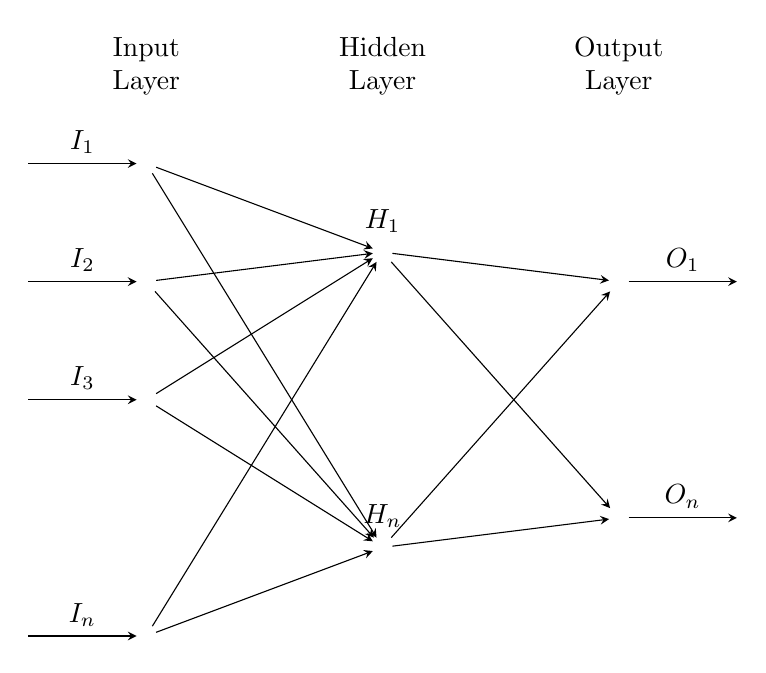
\begin{tikzpicture}[x=1.5cm, y=1.5cm, >=stealth]

    \foreach \m/\l [count=\y] in {1,2,3,missing,4}
    \node [every neuron/.try, neuron \m/.try] (input-\m) at (0,2.5-\y) {};

    \foreach \m [count=\y] in {1,missing,2}
    \node [every neuron/.try, neuron \m/.try ] (hidden-\m) at (2,2-\y*1.25) {};

    \foreach \m [count=\y] in {1,missing,2}
    \node [every neuron/.try, neuron \m/.try ] (output-\m) at (4,1.5-\y) {};

    \foreach \l [count=\i] in {1,2,3,n}
    \draw [<-] (input-\i) -- ++(-1,0)
    node [above, midway] {$I_\l$};

    \foreach \l [count=\i] in {1,n}
    \node [above] at (hidden-\i.north) {$H_\l$};

    \foreach \l [count=\i] in {1,n}
    \draw [->] (output-\i) -- ++(1,0)
    node [above, midway] {$O_\l$};

    \foreach \i in {1,...,4}
    \foreach \j in {1,...,2}
    \draw [->] (input-\i) -- (hidden-\j);

    \foreach \i in {1,...,2}
    \foreach \j in {1,...,2}
    \draw [->] (hidden-\i) -- (output-\j);

    \foreach \l [count=\x from 0] in {Input, Hidden, Output}
    \node [align=center, above] at (\x*2,2) {\l \\ Layer};

\end{tikzpicture}

    \caption[Aufbau]{Vereinfachter Aufbau eines Neuronales Netzwerk}
\end{wrapfigure}

In Abbildung 2 sieht man den Aufbau eines herkömmlichen künstlichen Neuronalen Netzwerks, so wie es noch vor 40 Jahren verwendet wurde. In der Grafik erkennt man drei Layer mit einer x-beliebigen Anzahl Neuronen, welche untereinander mit jeweils allen Neuronen der vorigen und nächsten Layer verbunden sind. Im Gegensatz zu einem biologischen Neuron, welches nur aktiv oder inaktiv sein kann, kann ein künstliches Neuron einen Zustand in Form eines Wertes von ${0 \leq x \leq 1}$ haben. Jede Verbindung hat einen Weight Paramter und auch jedes Neuron hat einen Bias. Die Anzahl der Hidden Layer kann an das Ziel angepasst und ausgewählt werden und auch die Anzahl der einzelnen Neuronen ist erstmal beliebig, als Faustregel für gute Ergebnisse gilt aber:

\begin{itemize}
    \item Die Anzahl der Neuronen in dem Hidden Layer sollte zwischen der Größe des Input und Output Layers liegen.
    \item Die Anzahl der Neuronen in dem Hidden Layer sollte etwa $\frac{2}{3}$ der Größe des Input Layers plus der Größe des Output Layers entsprechen.
    \item Die Anzahl der Neuronen in einem Hidden Layer sollte weniger als die Hälfte der Größe des Input Layers sein.\footnote{\cite[Alle drei Faustregeln]{heaton}}
\end{itemize}

\subsubsection{Erstellung eines Neuronalen Netzwerks anhand eines Beispiels}

Als Beispiel für ein Neuronales Netzwerk, welches darauf ausgelegt ist, geschriebene Ziffern aus Bildern mit 24x24 Pixeln und nur Graustufen zu erkennen wäre dann: Ein Input Layer mit $24^2$ Neuronen, jeweils für jeden Pixel, welche jeweils eine Aktivierung zwischen 0 (komplett weiß) und 1 (komplett schwarz) haben können, eines. Genau 10 Neuronen im Output Layer, für jedes Zahlzeichen eines. Schließlich muss die Anzahl der Hidden Layer und Neuronen festgelegt werden. Ich wähle als Beispiel 2 Layer mit jeweils 16 Neuronen, die Neuronen-Anzahl kann aber auch unterschiedlich sein. Auch die Weights und Biases werden zunächst zufällig ausgewählt, die Werte werden dann später im Trainingsprozess\footnote{siehe Kapitel \ref{backpropagation}} angepasst.

\subsection{Funktionsweise} \label{funktionsweise}

\begin{wrapfigure}{r}{75mm}
    \pgfplotsset{compat=1.16}
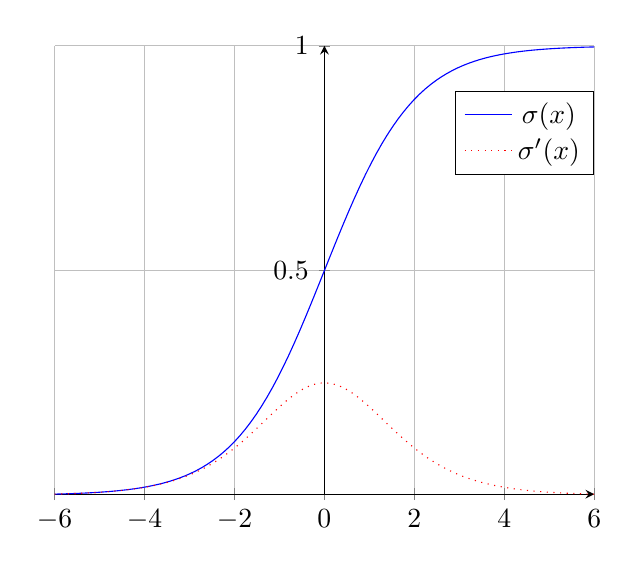
\begin{tikzpicture}[declare function={sigma(\x)=1/(1+exp(-\x));
sigmap(\x)=sigma(\x)*(1-sigma(\x));}]
\begin{axis}%
[
    grid=major,     
    xmin=-6,
    xmax=6,
    axis x line=bottom,
    ytick={0,.5,1},
    ymax=1,
    axis y line=middle,
    samples=100,
    domain=-6:6,
    legend style={at={(1,0.9)}}     
]
    \addplot[blue,mark=none]   (x,{sigma(x)});
    \addplot[red,dotted,mark=none]   (x,{sigmap(x)});
    \legend{$\sigma(x)$,$\sigma'(x)$}
\end{axis}
\end{tikzpicture}
    \caption[Sigmoid]{Die Sigmoidfunktion}
    \label{sigmoid}
\end{wrapfigure}


Ein Neuronales Netzwerk kann man sich eigentlich als eine große Mathematische Funktion vorstellen. In dem zuvor genannten Beispiel wäre es eine Funktion mit 576 Variablen und 10 Ergebnissen. Gibt man dieser Funktion nun ein Bild, beziehungsweise 576 Werte als Input, so werden von links nach rechts alle Weights $w$ und Biases $b$ zusammen mit dem vorigen Aktivierungswerten $a$ berechnet. Da ein Neuron aber nur Werte im Bereich $0\leq x \leq 1$ haben kann, so wird das Ergebniss noch mithilfe einer Aktivierungsfunktion in diesen Bereich umgewandelt. Eine früher Häufig verwendete Funktion ist dabei die Sigmoidfunktion, siehe Abbildung \ref{sigmoid}.\footnote{\cite{3blue1brown}} Es gibt aber auch noch eine Vielzahl weiterer Funktionen, wie die heute häufig verwendete ReLU Funktion\footnote{siehe Anhang \ref{anhang:weitereaktivierungsfunktionen}}, welche den Trainingprozess durch die einfachere Funktion beschleunigt.\footnote{\cite{nnfs} Seite 76 folgende} Die daraus resultierende Funktion würde in etwa so aussehen:\footnote{\cite{nnfs} Seite 185}

\begin{equation}\label{funktion1}
    \sigma(w_1a_1+w_2a_2+w_3a_3+ \ldots +w_na_n+b)
\end{equation}

Um mit dieser Formel alle Aktivierungen auf einmal berechnen zu können verwendet man folgende Funktion, in welcher alle Weights und Biases in Spalten-Vektoren zusammengefasst werden. Die Hochzeichen sind keine Exponenten sondern gelten als Bezeichnung für den Layer, hier beispielsweise 0 und 1. Das Ergebniss dieser Funktion ist ein Vektor mit allen Aktivierungen des darauf folgenden Layers.

\begin{equation}\label{funktion2}
    \sigma
    \begin{pmatrix}
        \begin{bmatrix}
            w_{0,0} & w_{0,1} & \ldots & w_{0,n} \\
            w_{1,0} & w_{1,1} & \ldots & w_{1,n} \\
            \vdots  & \vdots  & \ddots & \vdots  \\
            w_{k,0} & w_{k,1} & \ldots & w_{k,n}
        \end{bmatrix}
        \cdot
        \begin{bmatrix}
            a_0^{(0)} \\a_1^{(0)}\\\vdots\\a_n^{(0)}
        \end{bmatrix}
        +
        \begin{bmatrix}
            b_0 \\b_1\\\vdots\\b_k
        \end{bmatrix}
    \end{pmatrix}
    =
    a^{(1)}
\end{equation}\footnote{Gleichungen \ref{funktion2} und \ref{funktion3} von \cite{3blue1brown}}

Auch diese Funktion kann wiederrum kompakter formuliert werden und diese Schreibweise wird auch für gewöhnlich verwendet:

\begin{equation}\label{funktion3}
    a^{(1)}=\sigma(W\cdot a^{(0)}+b)
\end{equation}\footnotemark[20]%TODO ist die Zahl noch richtig?

Theoretisch wenn ein Neuron einen hohen Aktivierungswert haben soll, wenn beispielsweise eine gerade Linie erkannt wird (um mit anderen Neuronen zusammen im späteren Verlauf aus den Mustern ganze Ziffern zu erkennen), so müssen die Weights der zu dem Neuron führenden Verbindungen alle möglichst niedrige Aktivierungen haben, ausser an den Stellen an denen die Linie sich befinden soll. Um sicherzustellen, dass es sich wirklich um eine gerade Linie handelt befindet sich direkt über dem Strich ein Bereich in dem keine Aktivierungen sein sollten, dieser ist rot markiert. Das erkennt man in Abbildung \ref{examples} sehr gut. In a erkennt man die zu erkennende Linie und in b sieht man die zugehörigen Weights der Input Nodes zu dem Neuron. Dabei stellt grün positive Weights da, rot negative und Weiß/Transparent ist 0. Der Bias des Neurons stellt eine Zusätzliche Hürde oder eine Verstärkung da, was auch in Formel \ref{funktion1} als $b$ sichtbar ist.

\begin{figure}[H]
    \centering
    \subfloat[\centering Zu erkennendes Bild]{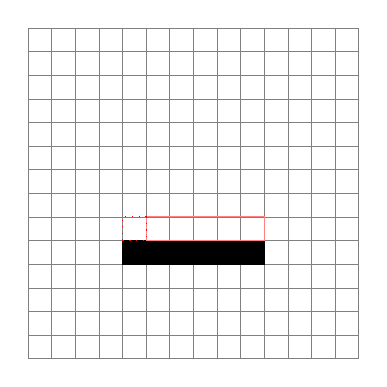
\begin{tikzpicture}
    \draw[step=3mm,gray,very thin] (0,0) grid (4.2,4.2);
    \filldraw[fill=black, draw=black] (1.2,1.2) rectangle (3,1.5);
    \filldraw[fill=none, draw=red!50!white] (1.5,1.5) rectangle (3,1.8);
    \filldraw[fill=none, draw=red, dotted] (1.2,1.5) rectangle (1.5,1.8);
\end{tikzpicture}}%
    \qquad
    \subfloat[\centering Benötigte Weights]{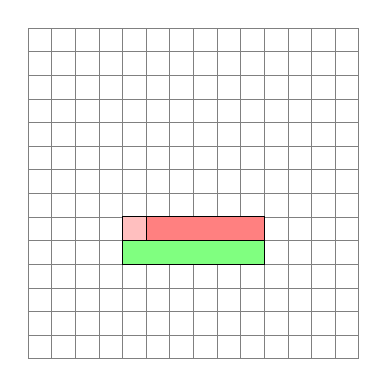
\begin{tikzpicture}
    \draw[step=3mm,gray,very thin] (0,0) grid (4.2,4.2);
    \filldraw[fill=green!50!white, draw=black] (1.2,1.2) rectangle (3,1.5);
    \filldraw[fill=red!50!white, draw=black] (1.5,1.5) rectangle (3,1.8);
    \filldraw[fill=red!25!white, draw=black] (1.2,1.5) rectangle (1.5,1.8);
\end{tikzpicture}}
    \caption[Visualisierung]{Visualisierung der gewünschten Formen a und die dazugehörigen Weights b (jeweils abgeschnitten)}
    \label{examples}%
\end{figure}

\subsubsection{Trainieren - Backpropagation} \label{backpropagation}

Dieser Prozess ist der wichtigste. Durch das Trainieren erzielt ein Neuronales Netzwerk den Effekt des selbstständigen Lernens. Und da die Werte der Weights und Biases zunächst zufällig ausgewählt wurden, muss das Netzwerk trainiert werden um nicht völligen Unsinn auszugeben.

Um herauszufinden wie gut oder schlecht ein Neuronales Netzwerk arbeitet, also auf das Beispiel bezogen wie genau oder ungenau es Ziffern erkennen kann, gibt es die Cost Function. Es gibt verschiedene Arten und Möglichkeiten ähnliche Funktionen anzuwenden, hier werde ich mich allerdings auf die Minimalisierung der Cost Function beziehen. Diese Funktion ergibt sich aus den Ergebnissen des Netzwerks aus den Trainingsdaten und allen Werten der Weights und Biases. Als Ergebniss kommt eine einzige Zahl heraus welche hoch ist, wenn das Netzwerk schlechte Ergebnisse erzielt und gegen 0 läuft, wenn das Netzwerk sehr gute Ergebnisse liefert. Es geht also darum

\begin{equation}\label{costfunction}
    costfunction
\end{equation}

%\footnote{Ein Code Beispiel, wie man ein solches Netzwerk mit modernen Frameworks erstellen und trainieren würde befindet sich im Anhang \ref{anhang:colab1}.}
%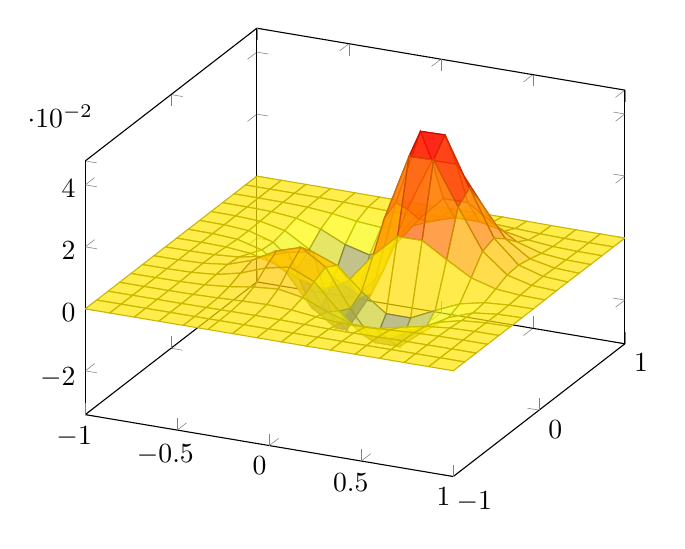
\begin{tikzpicture}
    \begin{axis}[domain=-1:1, y domain=-1:1,  colormap/hot,samples=16]
        \addplot3[surf, fill opacity=0.7,] {x*y*exp(x+2*y-9*x^2-9*y^2)};
    \end{axis}
\end{tikzpicture}